\subsection{Environnement de travail}
%------------------------------------------------------------------------------
\begin{frame}\frametitle{Méthode agile}
\centering
\begin{minipage}[c]{.5\linewidth}
	\begin{beamerboxesrounded}[shadow=true]{Gestion de projet}
		
\includegraphics[width=\linewidth]{../image/lighthouseLogo.png}
	\end{beamerboxesrounded}
\end{minipage}
\vfill
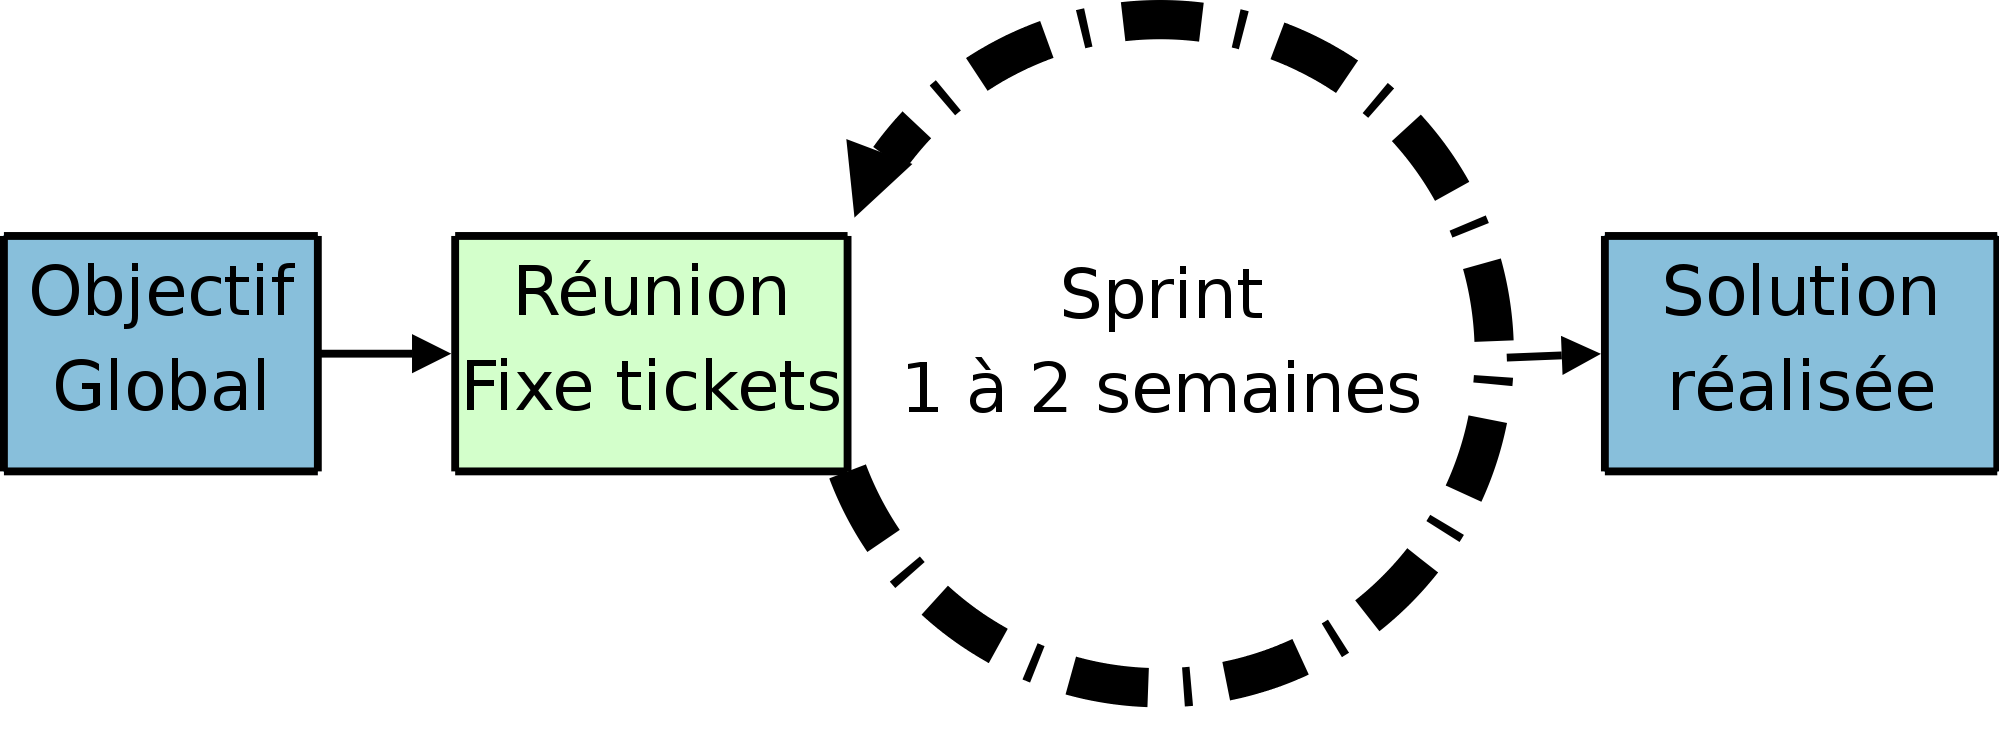
\includegraphics[width=1\linewidth]{../image/agileDev.png}
\end{frame}
%------------------------------------------------------------------------------
\begin{frame}\frametitle{Gestion des sources}
\begin{centering}
	\begin{minipage}[c]{.6\linewidth}
		\begin{beamerboxesrounded}[shadow=true,center]{Gestionnaire de version}
			\centering
			
\includegraphics[width=.4\linewidth]{../image/gitLogo.png}\hfil
		\end{beamerboxesrounded}
	\end{minipage}
	\vfill
	\begin{minipage}[c]{.6\linewidth}
		\begin{beamerboxesrounded}[shadow=true,center]{Hébergement de dépôt}
			\centering
			
\includegraphics[width=.3\linewidth]{../image/githubLogo.png}
		\end{beamerboxesrounded}
	\end{minipage}
	\vfill
\end{centering}
\end{frame}
%------------------------------------------------------------------------------
\begin{frame}\frametitle{Fonctionnement}
\begin{centering}
\begin{minipage}[c]{.5\linewidth}
	\begin{beamerboxesrounded}[shadow=true,center]{Subversion}
		\centering
		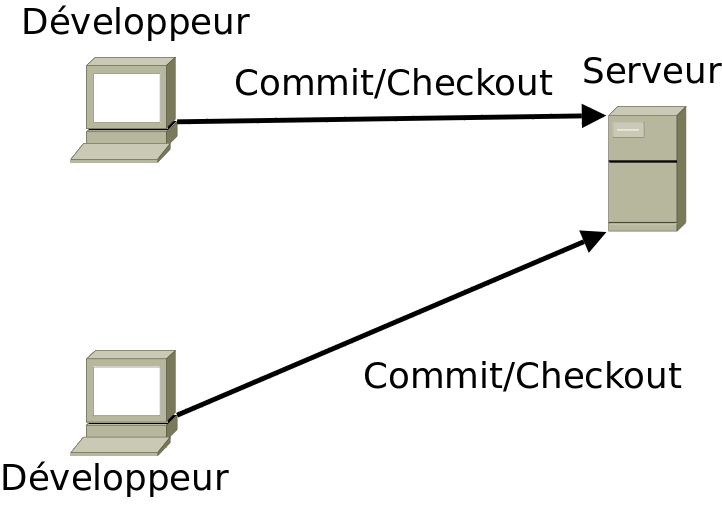
\includegraphics[width=\linewidth]{../image/svn.png}
	\end{beamerboxesrounded}
\end{minipage}
\vfill
\begin{minipage}[c]{.5\linewidth}
 	\begin{beamerboxesrounded}[shadow=true,center]{Git}
	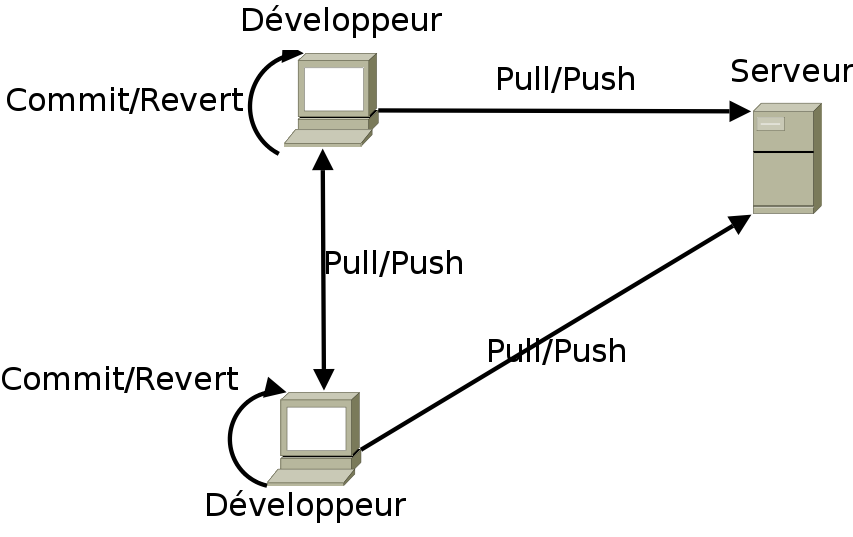
\includegraphics[width=\linewidth]{../image/gitSimplifie.png}
 	\end{beamerboxesrounded}
\end{minipage}
\vfill
\end{centering}
\end{frame}
%------------------------------------------------------------------------------
\begin{frame}\frametitle{Outil de travail}
\begin{centering}
	\begin{minipage}[c]{.6\linewidth}
		\begin{beamerboxesrounded}[shadow=true,center]{Environnement de développement}
			\centering
			
\includegraphics[width=.4\linewidth]{../image/intellijLogo.png}
		\end{beamerboxesrounded}
	\end{minipage}
	\vfill
	\begin{minipage}[c]{.6\linewidth}
		\begin{beamerboxesrounded}[shadow=true,center]{Outil de profiling}
			\centering
			
\includegraphics[width=.3\linewidth]{../image/yourkit.jpg}
		\end{beamerboxesrounded}
	\end{minipage}
	\vfill

\end{centering}
\end{frame}
%------------------------------------------------------------------------------
\subsection{Transition}
\begin{frame}
\frametitle{Transition vers JAXP}
\begin{minipage}[c]{\linewidth}
	\begin{beamerboxesrounded}[shadow=true]{XMLWriter et XMLParser}
		\begin{itemize}
			\item Traité au cas par cas
			\item Création de nouveau XMLWriter et XMLParser
		\end{itemize}
	\end{beamerboxesrounded}
\end{minipage}
\vfill
\begin{minipage}[c]{\linewidth}
	\begin{beamerboxesrounded}[shadow=true]{XMLElement}
		\begin{itemize}
			\item Extraction de l'interface
			\item Nouvelle implémentation
		\end{itemize}
	\end{beamerboxesrounded}
\end{minipage}
\vfill
\end{frame}
%------------------------------------------------------------------------------
\begin{frame}
\frametitle{Patron de conception adaptateur}
\hfil
\begin{minipage}[c]{.3\linewidth}
	\begin{beamerboxesrounded}[shadow=true]{Sans adaptateur}
		\centering
		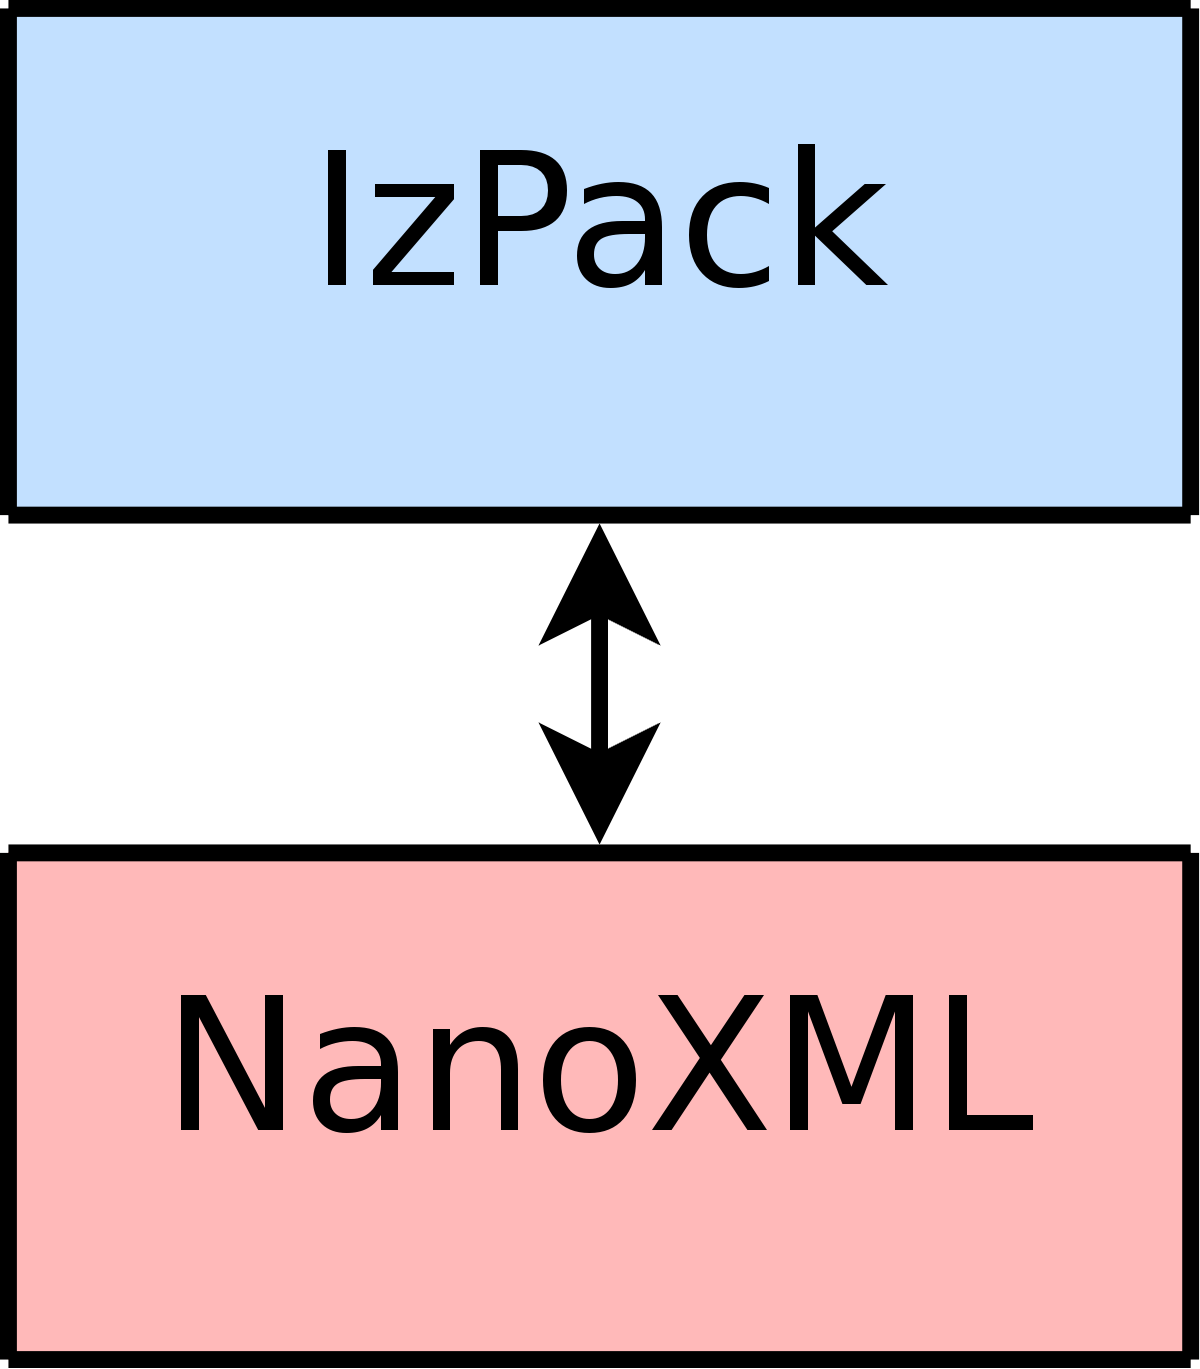
\includegraphics[width=.8\linewidth]{../image/sansAdaptateur.png}
	\end{beamerboxesrounded}
\end{minipage}
\hfil
\begin{minipage}[c]{.3\linewidth}
	\begin{beamerboxesrounded}[shadow=true]{Avec adaptateur}
		\centering
		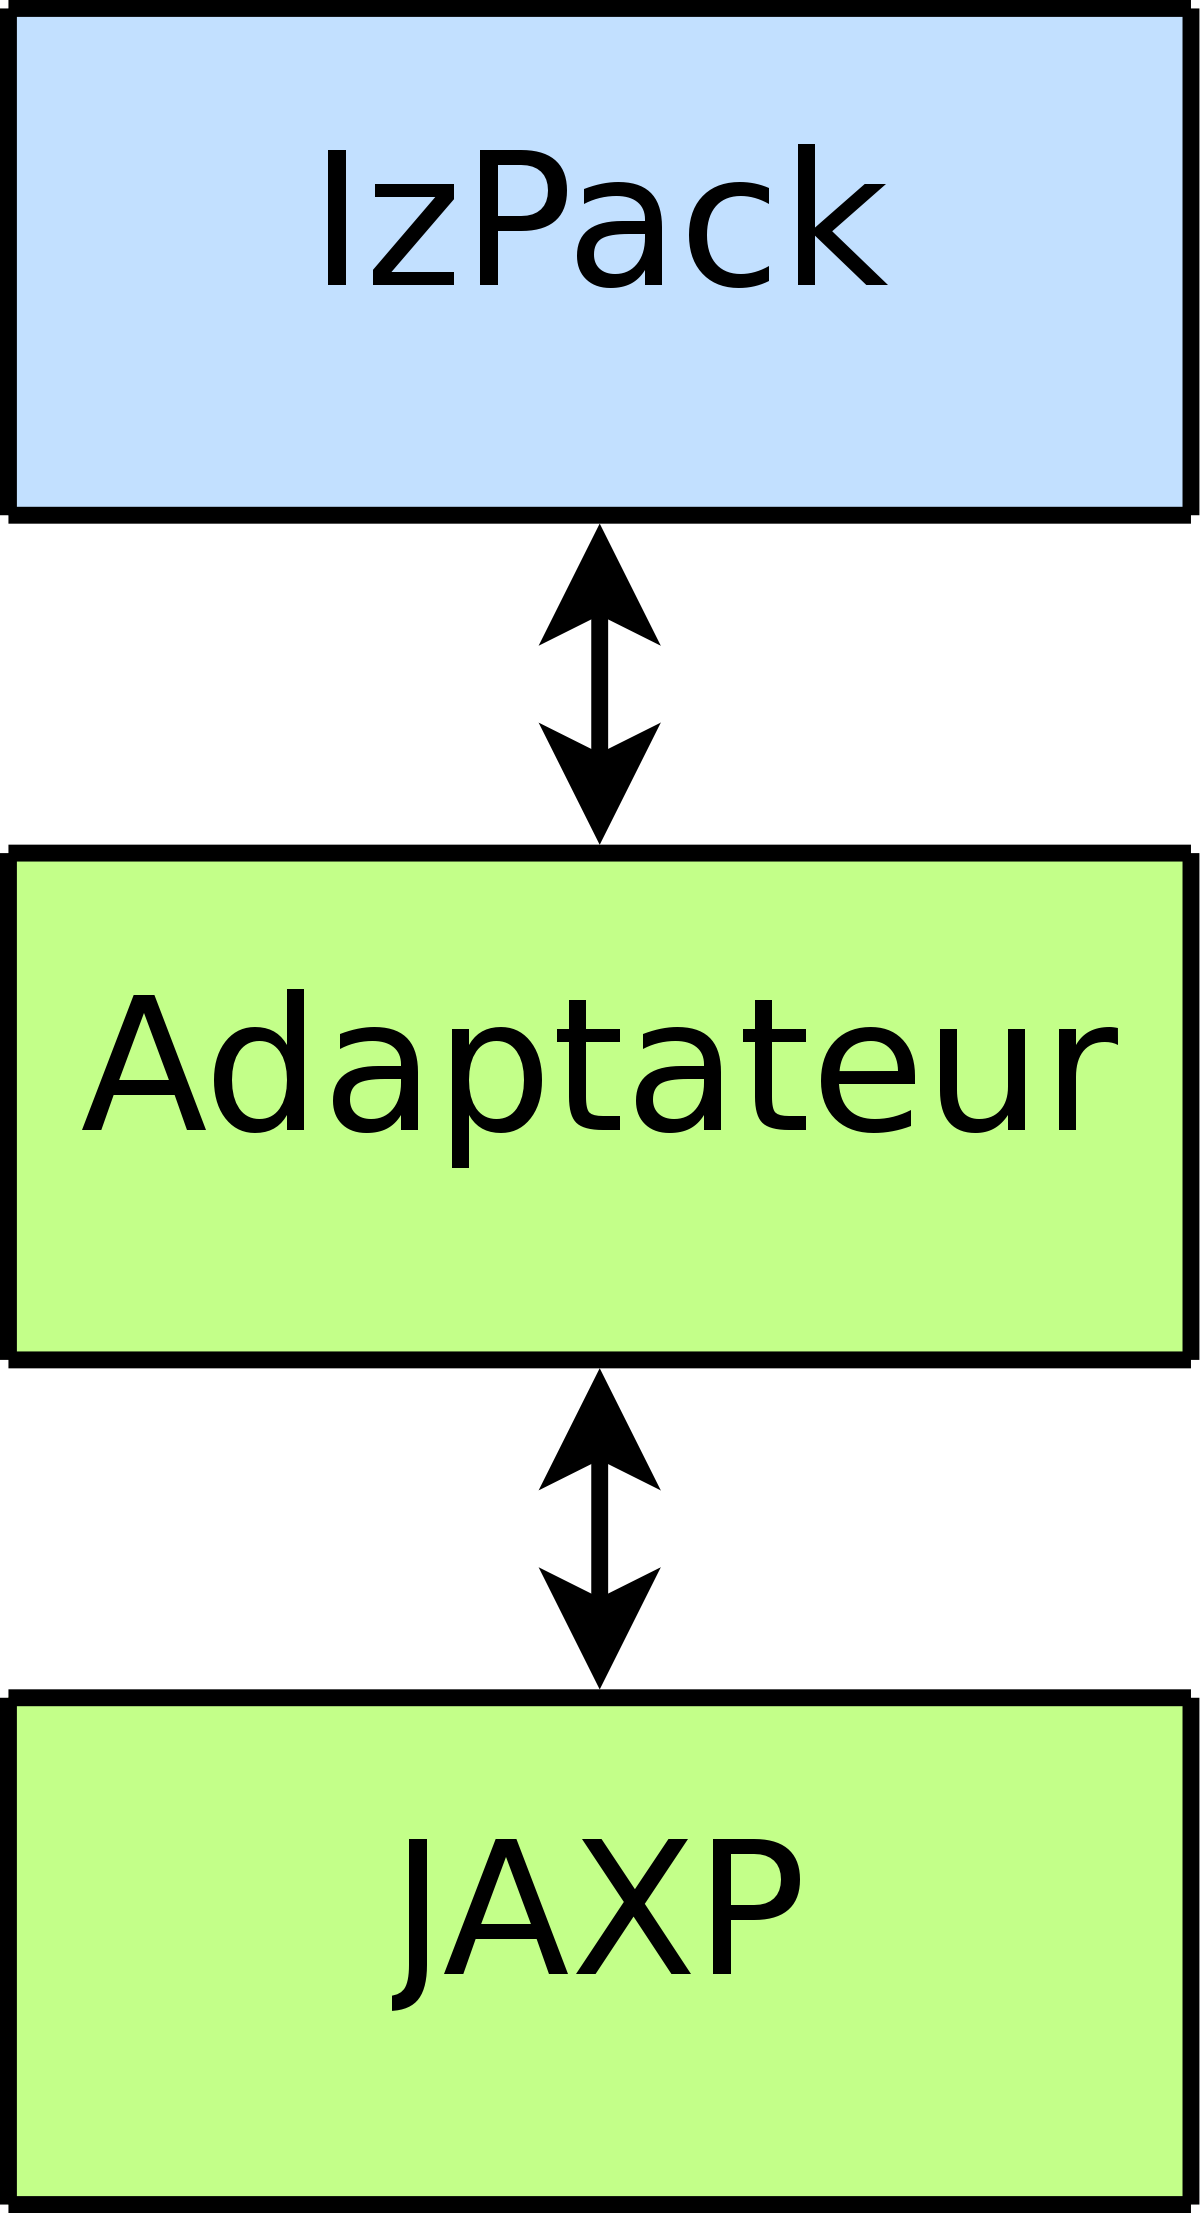
\includegraphics[width=.8\linewidth]{../image/avecAdaptateur.png}
	\end{beamerboxesrounded}
\end{minipage}
\hfil
\vfill
\begin{minipage}[c]{\linewidth}
	\begin{beamerboxesrounded}[shadow=true]{Avantages}
	\begin{itemize}
		\item Changements minimes
		\item Intégration rapide
		\item Logique centralisée
	\end{itemize}
	\end{beamerboxesrounded}
\end{minipage}
\vfill
\end{frame}
%------------------------------------------------------------------------------
\subsection{Tests}
\begin{frame}\frametitle{Tests effectués}
\begin{minipage}[c]{.9\linewidth}
	\begin{beamerboxesrounded}[shadow=true]{Tests unitaires comparatifs}
		\begin{itemize}
			\item Adaptateur <-> NanoXML
			\item Assurent un comportement identique
		\end{itemize}
	\end{beamerboxesrounded}
\end{minipage}
\vfill
\begin{minipage}[c]{.9\linewidth}
	\begin{beamerboxesrounded}[shadow=true]{Tests fonctionnels}
		\begin{itemize}
			\item Intégration de la solution
			\item Génération d'installateur
		\end{itemize}
	\end{beamerboxesrounded}
\end{minipage}
\end{frame}
%------------------------------------------------------------------------------
\begin{frame}\frametitle{Installation de IzPack}
	\centering
	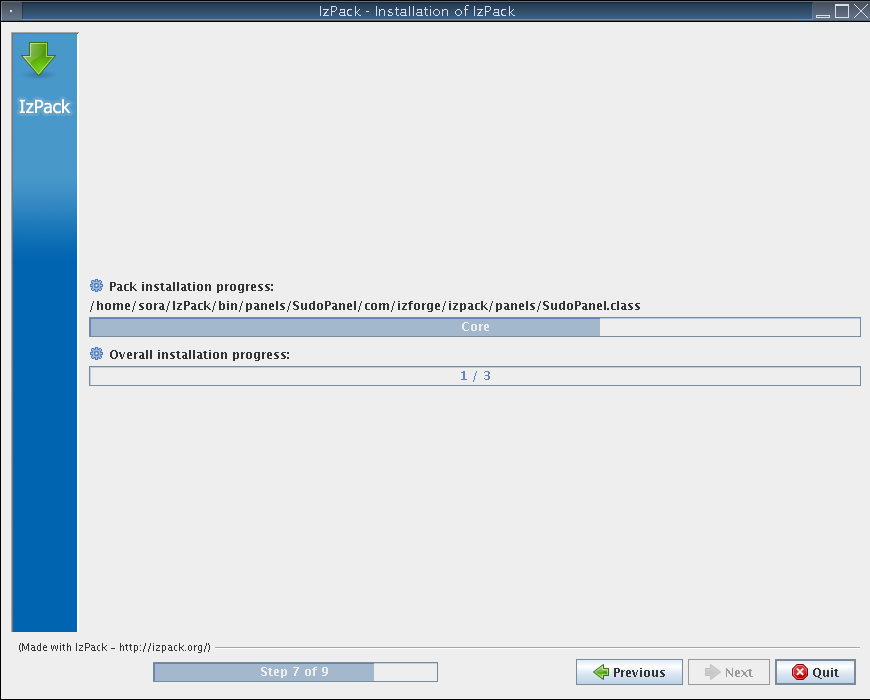
\includegraphics[width=\linewidth]{../image/installationIzpack.png}
\end{frame}
%------------------------------------------------------------------------------
\begin{frame}\frametitle{Installation de Glassfish}
	\centering
	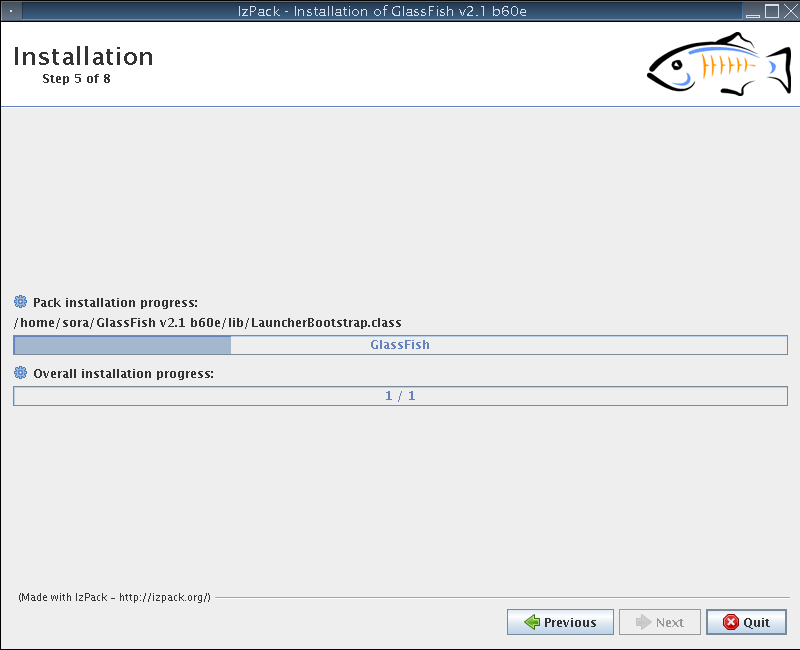
\includegraphics[width=\linewidth]{../image/installationGlassfish.png}
\end{frame}
%------------------------------------------------------------------------------
\subsection{Principaux problèmes rencontrés}
\begin{frame}\frametitle{Problème : Synchronisation des sources}
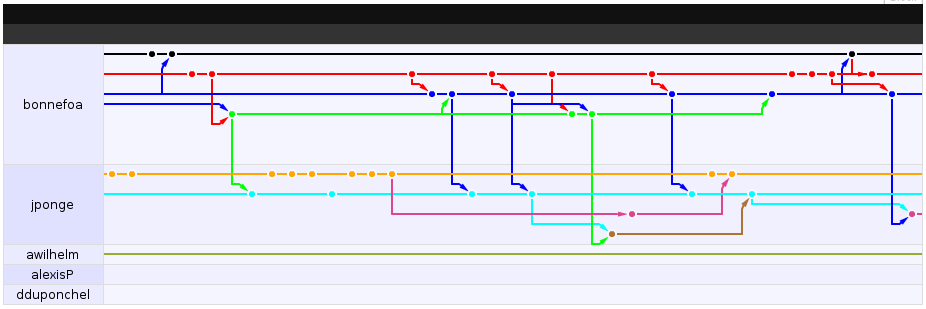
\includegraphics[width=\linewidth]{../image/gitHubBranche.png}
\end{frame}
%------------------------------------------------------------------------------
\begin{frame}[containsverbatim]\frametitle{Différences DOM, NanoXML}
\begin{centering}
\begin{minipage}[c]{.5\linewidth}
\begin{verbatim}
<root>
  <child/>
</root>
\end{verbatim}
\end{minipage}
\vfill
\begin{minipage}[c]{.4\linewidth}
	\begin{beamerboxesrounded}[shadow=true]{NanoXML}
		1  enfant
	\end{beamerboxesrounded}
\end{minipage}
\hfill
\begin{minipage}[c]{.4\linewidth}
	\begin{beamerboxesrounded}[shadow=true]{DOM}
		3  enfant
	\end{beamerboxesrounded}
\end{minipage}
\vfill
\end{centering}
\end{frame}
%------------------------------------------------------------------------------
\begin{frame}\frametitle{XInclude}
\end{frame}
%------------------------------------------------------------------------------
\begin{frame}\frametitle{Numéro de lignes}
\end{frame}